\documentclass[border=3pt]{standalone}
% Preâmbulo compartilhado pelos diagramas TikZ da aula 8 de IHR (Métodos de Pesquisa)
\usepackage[T1]{fontenc}
\usepackage[utf8]{inputenc}
\usepackage{lmodern}
\usepackage{amsmath}
\usepackage{xcolor}
\usepackage{tikz}
\usetikzlibrary{arrows.meta,angles,quotes,decorations.pathmorphing,decorations.pathreplacing,calc,
                positioning,shapes.geometric,shapes.misc,backgrounds,fit,
                math}

% Paleta (mesma dos SVGs originais)
% Paleta da disciplina de IHR: acento azul (#1A6FB5), cor de destaque do tema.
% (o nome "dblue" é mantido para não alterar todos os diagramas)
\definecolor{dblue}{HTML}{1A6FB5}
\definecolor{dorange}{HTML}{B3541E}
\definecolor{dgreen}{HTML}{4A7C59}
\definecolor{dred}{HTML}{9C4B4B}
\definecolor{dcream}{HTML}{F4F1EA}
\definecolor{dshade}{HTML}{DDD7C9}

% Função gaussiana (não normalizada por padrão de escala visual)
\pgfmathdeclarefunction{gauss}{3}{%
  \pgfmathparse{1/(#3*sqrt(2*pi))*exp(-((#1-#2)^2)/(2*#3^2))}%
}

% Estilos comuns (prefixo d... para não colidir com chaves internas do pgf)
\tikzset{
  >={Stealth[length=2mm]},
  dguide/.style={gray!55, dashed, line width=0.4pt},
  daxis/.style={gray!60, line width=0.7pt, ->},
  dbody/.style={fill=black!3, draw=black!80, line width=1pt},
  dacc/.style={draw=dblue, line width=1pt},
  dlbl/.style={black!55, font=\small},
  dsub/.style={black!45, font=\footnotesize},
  dstate/.style={circle, draw=black!80, fill=dcream, line width=1pt,
                 minimum size=17mm, font=\large, inner sep=1pt},
  dobs/.style={circle, draw=black!80, fill=dshade, line width=1pt,
               minimum size=14mm, font=\large, inner sep=1pt},
  dbox/.style={rounded corners=2pt, draw=black!80, fill=dcream, line width=1pt,
               align=center, inner sep=6pt},
  dop/.style={circle, draw=black!80, fill=white, line width=1pt,
              minimum size=6mm, inner sep=0pt, font=\small},
  dtrans/.style={->, dblue, line width=1pt},
  dmeas/.style={->, dorange, line width=1pt},
  dcurve/.style={line width=1pt, dblue},
  dcurveb/.style={line width=1.4pt, dorange},
}

\begin{document}
\hyphenpenalty=10000 \exhyphenpenalty=10000 \tolerance=9999 \emergencystretch=3em
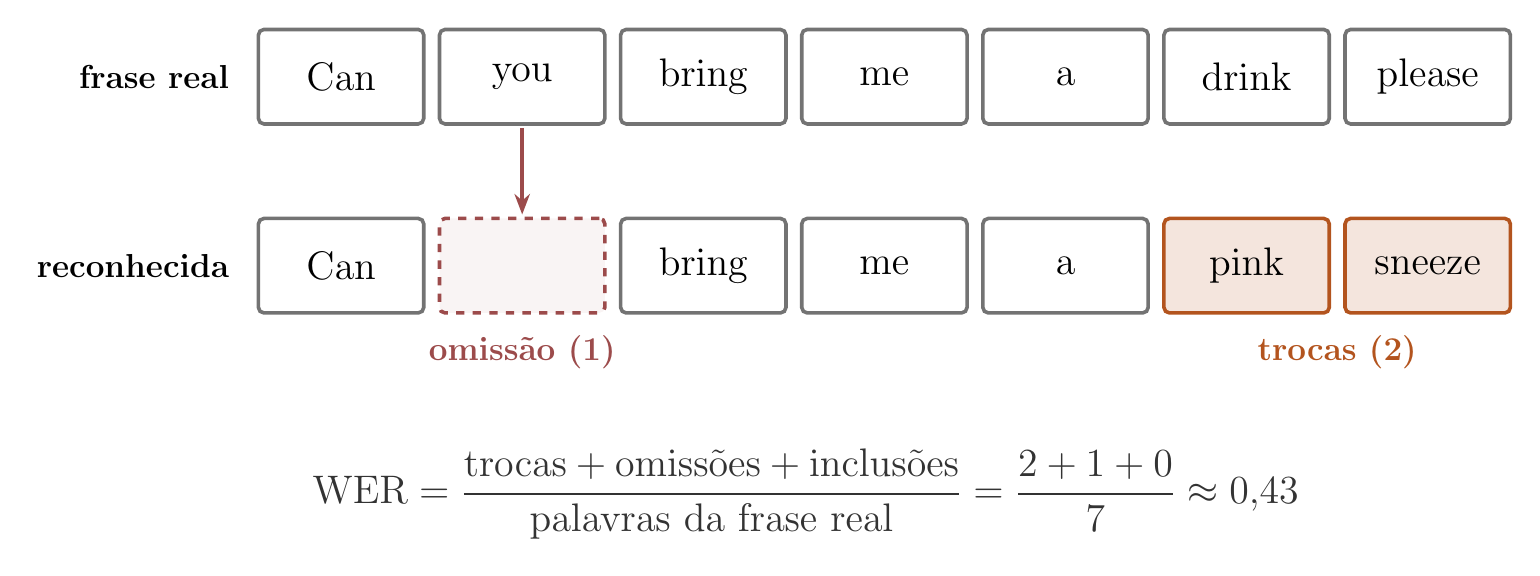
\begin{tikzpicture}[x=1cm,y=1cm]
  \tikzset{w/.style={dbox, minimum width=2.1cm, minimum height=1.2cm, font=\Large, line width=1.3pt, inner sep=3pt}}
  \node[font=\large\bfseries, anchor=east] at (3.3,6.0) {frase real};
  \node[font=\large\bfseries, anchor=east] at (3.3,3.6) {reconhecida};
  \foreach \i/\t in {1/Can,2/you,3/bring,4/me,5/a,6/drink,7/please} {\node[w, draw=black!55, fill=white] at ({4.6+(\i-1)*2.3},6.0) {\t};}
  \foreach \i/\t in {1/Can,3/bring,4/me,5/a} {\node[w, draw=black!55, fill=white] at ({4.6+(\i-1)*2.3},3.6) {\t};}
  \node[w, draw=dred, dashed, fill=dred!6] at ({4.6+1*2.3},3.6) {};
  \node[w, draw=dorange, fill=dorange!15] at ({4.6+5*2.3},3.6) {pink};
  \node[w, draw=dorange, fill=dorange!15] at ({4.6+6*2.3},3.6) {sneeze};
  \draw[dred, line width=1.4pt, -{Stealth[length=2.6mm]}] ({4.6+1*2.3},5.35) -- ({4.6+1*2.3},4.25);
  \node[font=\large\bfseries, dred] at ({4.6+1*2.3},2.5) {omissão (1)};
  \node[font=\large\bfseries, dorange] at ({4.6+5.5*2.3},2.5) {trocas (2)};
  \node[font=\Large, black!80] at (10.5,0.7) {$\mathrm{WER}=\dfrac{\text{trocas}+\text{omissões}+\text{inclusões}}{\text{palavras da frase real}}=\dfrac{2+1+0}{7}\approx 0{,}43$};
\end{tikzpicture}
\end{document}
